\begin{figure}[t]
	\centerline{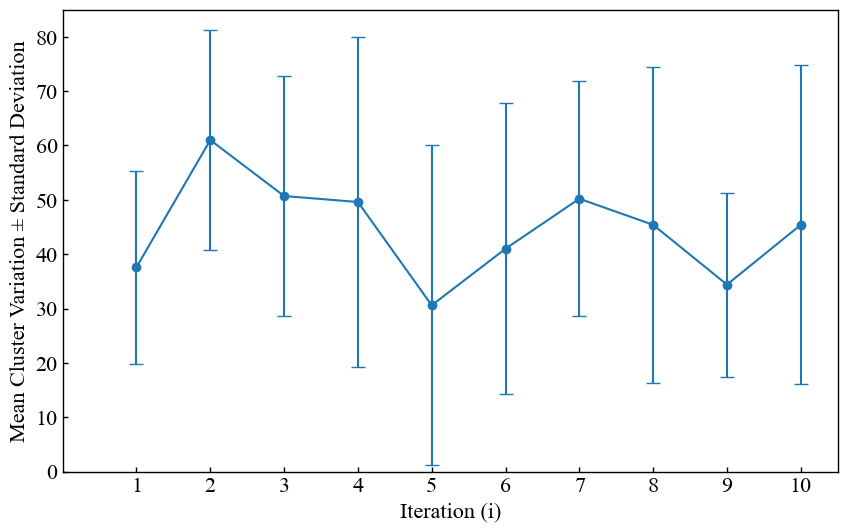
\includegraphics[width=\linewidth]{img/clustering.png}}
	\caption{Stability verification of cluster assignment for short video dataset}
	\label{fig:clustering-stability}
\end{figure}

%
Section~\ref{subsec:evaluation-short} demonstrated that three-dimensional point-cloud features are effective for activity-level estimation.
Clustering instability may partially explain the limited accuracy improvement from multiple features.
K-means clustering ($k$=3) was applied to the short-video dataset as a baseline.
One sample was randomly removed and clustering was re-run 10 times per trial, repeated over 10 trials.
Fig.~\ref{fig:clustering-stability} shows the number of changed cluster assignments.
Cluster changes ranged from approximately 20 to 40 per trial.
Clustering instability is a contributing factor to the limited accuracy improvement from multiple features.
The XGBoost all-feature model achieved the highest accuracy in Section~\ref{subsec:evaluation-short}.
The accuracy gain over single-feature models remained limited.
A baseline clustering result was established with k-means ($k$=3) on the full dataset.
Mean and standard deviation of reassignment counts were computed across 10 trials of 10 removal-and-reclustering operations.
Fig.~\ref{fig:clustering-stability} plots the mean and standard deviation on the vertical axis against trial number on the horizontal axis.
